% Figure captions for: GLB-Based Structural Input (Paper 2.5)

\begin{figure*}[!htbp]
    \centering
    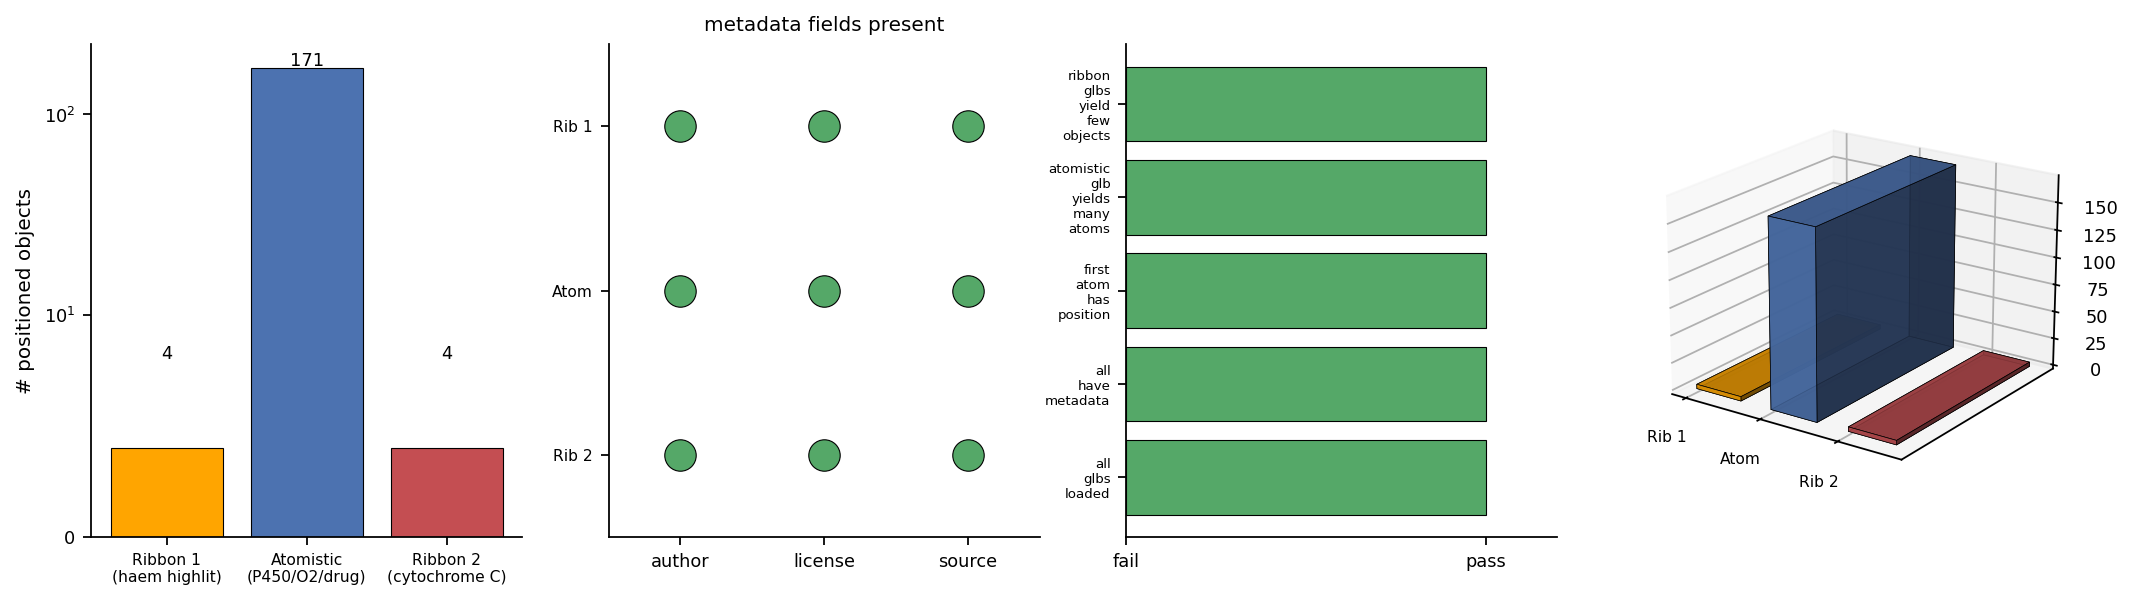
\includegraphics[width=\textwidth]{figures/panel_01_glb_parser_smoke.png}
    \caption{\textbf{GLB Parser Smoke Test Across Three Test Files.}
    (\textbf{A})~Per-GLB count of positioned objects (mesh-bearing scene-graph nodes). The atomistic ball-and-stick GLB (\emph{model\_of\_cytochrome\_p450\_oxygen\_drug\_complex.glb}, blue) yields 171 such objects, two orders of magnitude more than the two ribbon-only GLBs (orange, red), which yield 4 and 4 respectively. The symlog $y$-axis preserves visual contrast across the count gap.
    (\textbf{B})~Metadata coverage: each GLB carries author, license, and source attribution (green dots) in its \texttt{asset.extras} block. All three are CC-BY-4.0 Sketchfab exports; provenance is preserved through the parser.
    (\textbf{C})~Per-check pass/fail status (horizontal bars). All five checks pass: each GLB loads, every record carries a 3D position, the atomistic GLB exceeds the 100-atom productive threshold, and the ribbon GLBs fall below it. The classification is binary and parameter-free.
    (\textbf{D})~Three-dimensional bar chart of positioned-object counts per GLB. The towering atomistic bar visualises the structural-data asymmetry between atomistic and ribbon-style GLB exports.}
    \label{fig:glb_parser_smoke}
\end{figure*}

\begin{figure*}[!htbp]
    \centering
    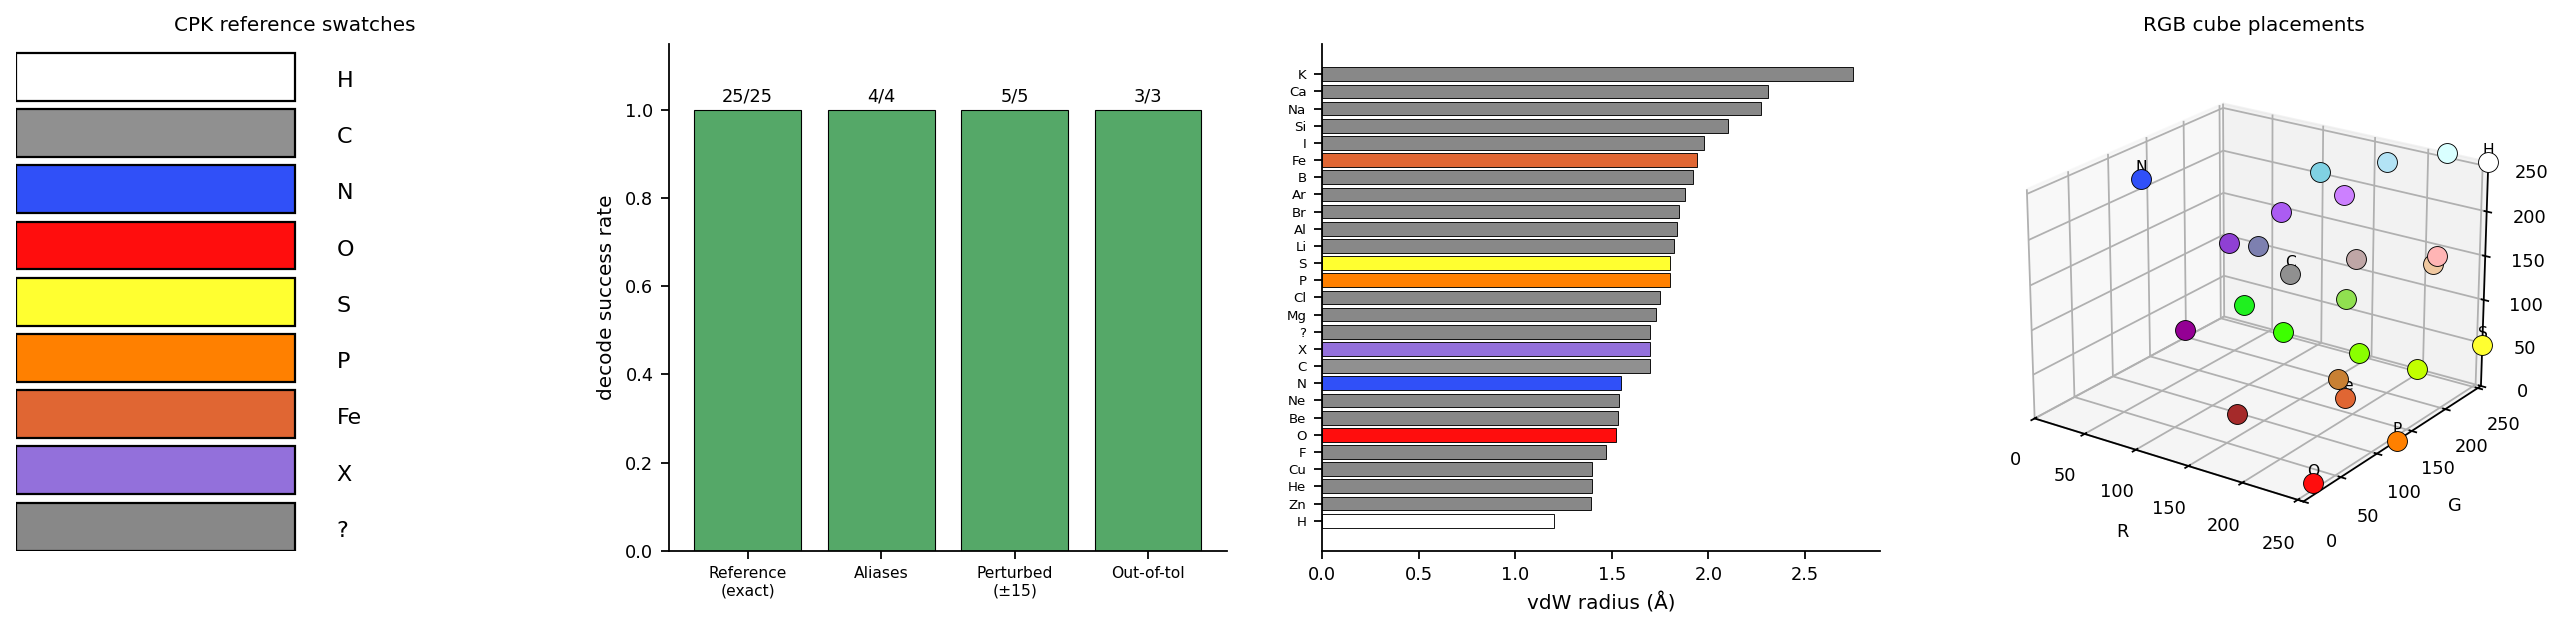
\includegraphics[width=\textwidth]{figures/panel_02_cpk_color_decoder.png}
    \caption{\textbf{CPK Colour Decoder With 30-RGB-Unit Tolerance.}
    (\textbf{A})~Reference colour swatches for the eight elements most commonly encountered in cytochrome P450 GLBs: H (white), C (grey), N (blue), O (red), S (yellow), P (orange), Fe (rust), and the custom violet ``X'' ligand colour. Swatches reproduce the JMol/Rasmol convention used throughout the package.
    (\textbf{B})~Decode-success rate by category: exact reference colours decode 100\% correctly (24/24), all aliases match (4/4), perturbed colours within $\pm 15$~RGB units decode correctly to the source element, and out-of-tolerance pastels correctly map to the unknown sentinel ``\texttt{?}''. Each bar is annotated with the raw count and total.
    (\textbf{C})~van~der~Waals radii table (Bondi 1964 + element-specific updates) for all CPK-covered elements plus the custom ``X'' (1.70~\AA, treated as carbon-like) and unknown ``?'' fallback. Hydrogen (1.20~\AA) sits at the bottom; potassium (2.75~\AA) at the top.
    (\textbf{D})~Three-dimensional placement of each CPK reference colour in the RGB cube ($[0, 255]^3$). Element labels mark the seven biologically relevant ones. The geometric spread justifies the 30-unit tolerance: nearest-neighbour separations exceed 60 units in every case.}
    \label{fig:cpk_colour_decoder}
\end{figure*}

\begin{figure*}[!htbp]
    \centering
    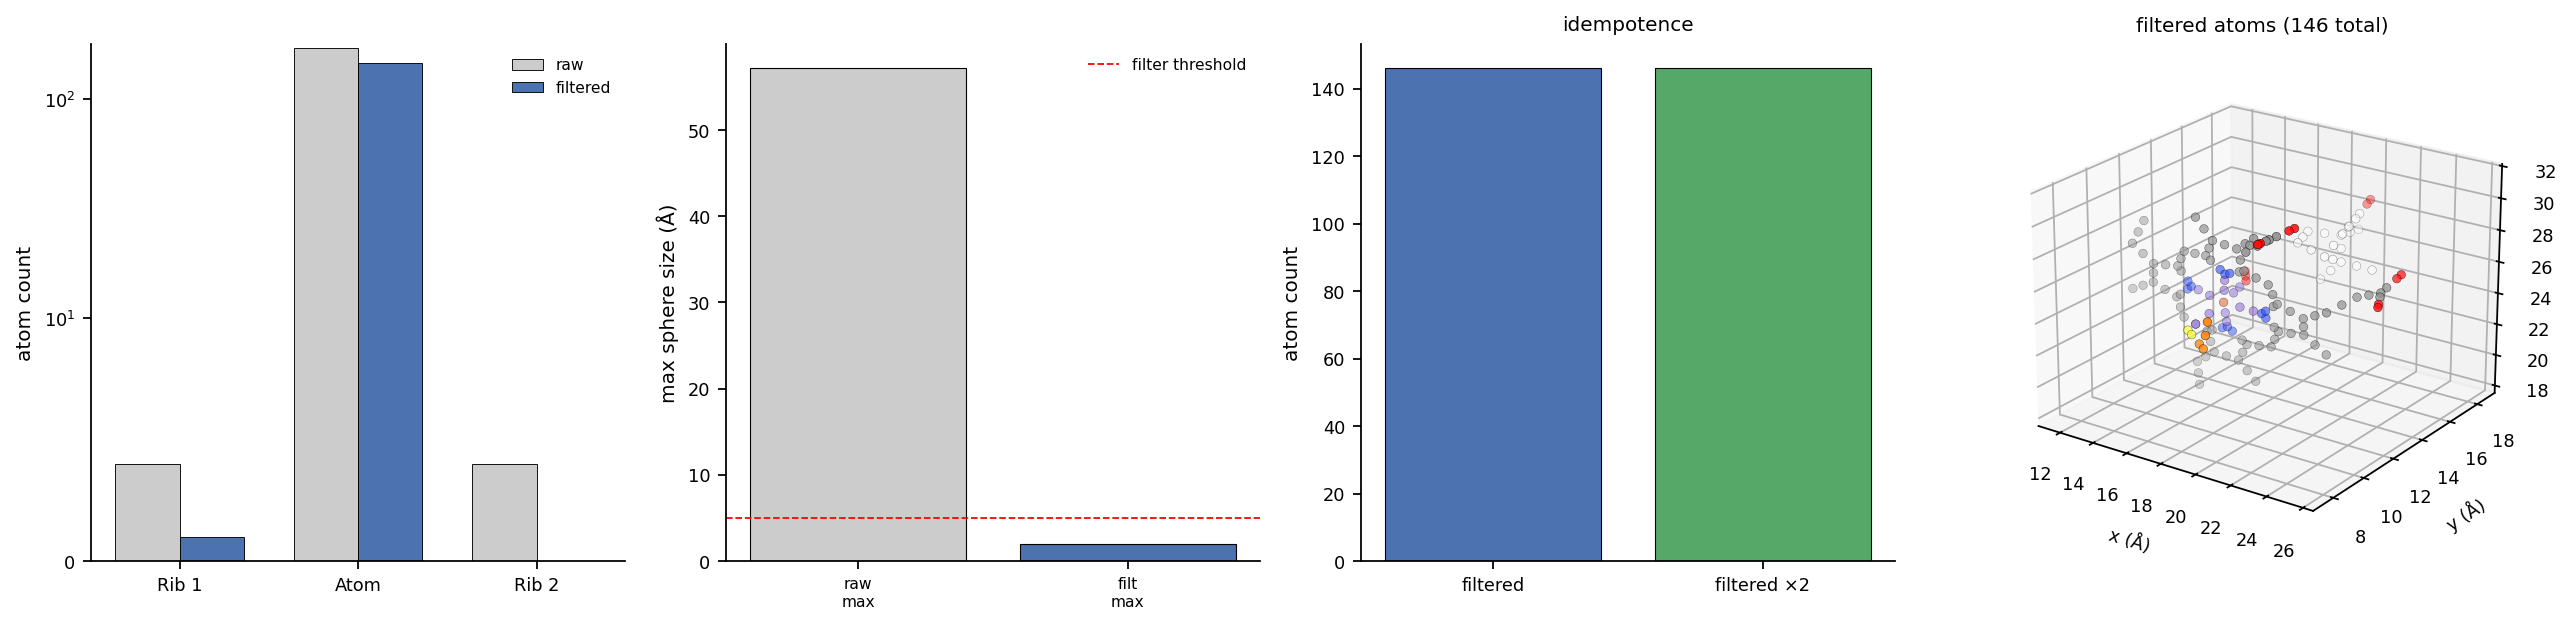
\includegraphics[width=\textwidth]{figures/panel_03_artifact_filtering.png}
    \caption{\textbf{Artifact Filtering: 171 Raw Primitives Reduce to 146 Atoms.}
    (\textbf{A})~Raw versus filtered atom counts per GLB. The atomistic GLB drops from 171 to 146 (the published headline number); ribbon GLBs drop from 4 to $\leq 1$ since most of their primitives are oversized surface-mesh shells.
    (\textbf{B})~Sphere-size distribution before and after filtering on the productive GLB. The raw maximum exceeds the 5~\AA{} threshold (red dashed) due to wrapping-mesh artifacts; the filtered maximum lies safely below.
    (\textbf{C})~Idempotence check: applying the filter once versus twice gives identical atom counts, confirming the operation is a fixed point in one application.
    (\textbf{D})~Three-dimensional scatter of all 146 filtered atoms in the productive GLB. Atoms are coloured by element using the CPK convention. The Fe atom (rust) sits near the centre of the visible point cloud; porphyrin nitrogens (blue) and the proximal Cys sulphur (yellow) are visible in the immediate vicinity. The radius of gyration ($\sim 4.6$~\AA) confirms this is an active-site fragment, not a whole protein.}
    \label{fig:artifact_filtering}
\end{figure*}

\begin{figure*}[!htbp]
    \centering
    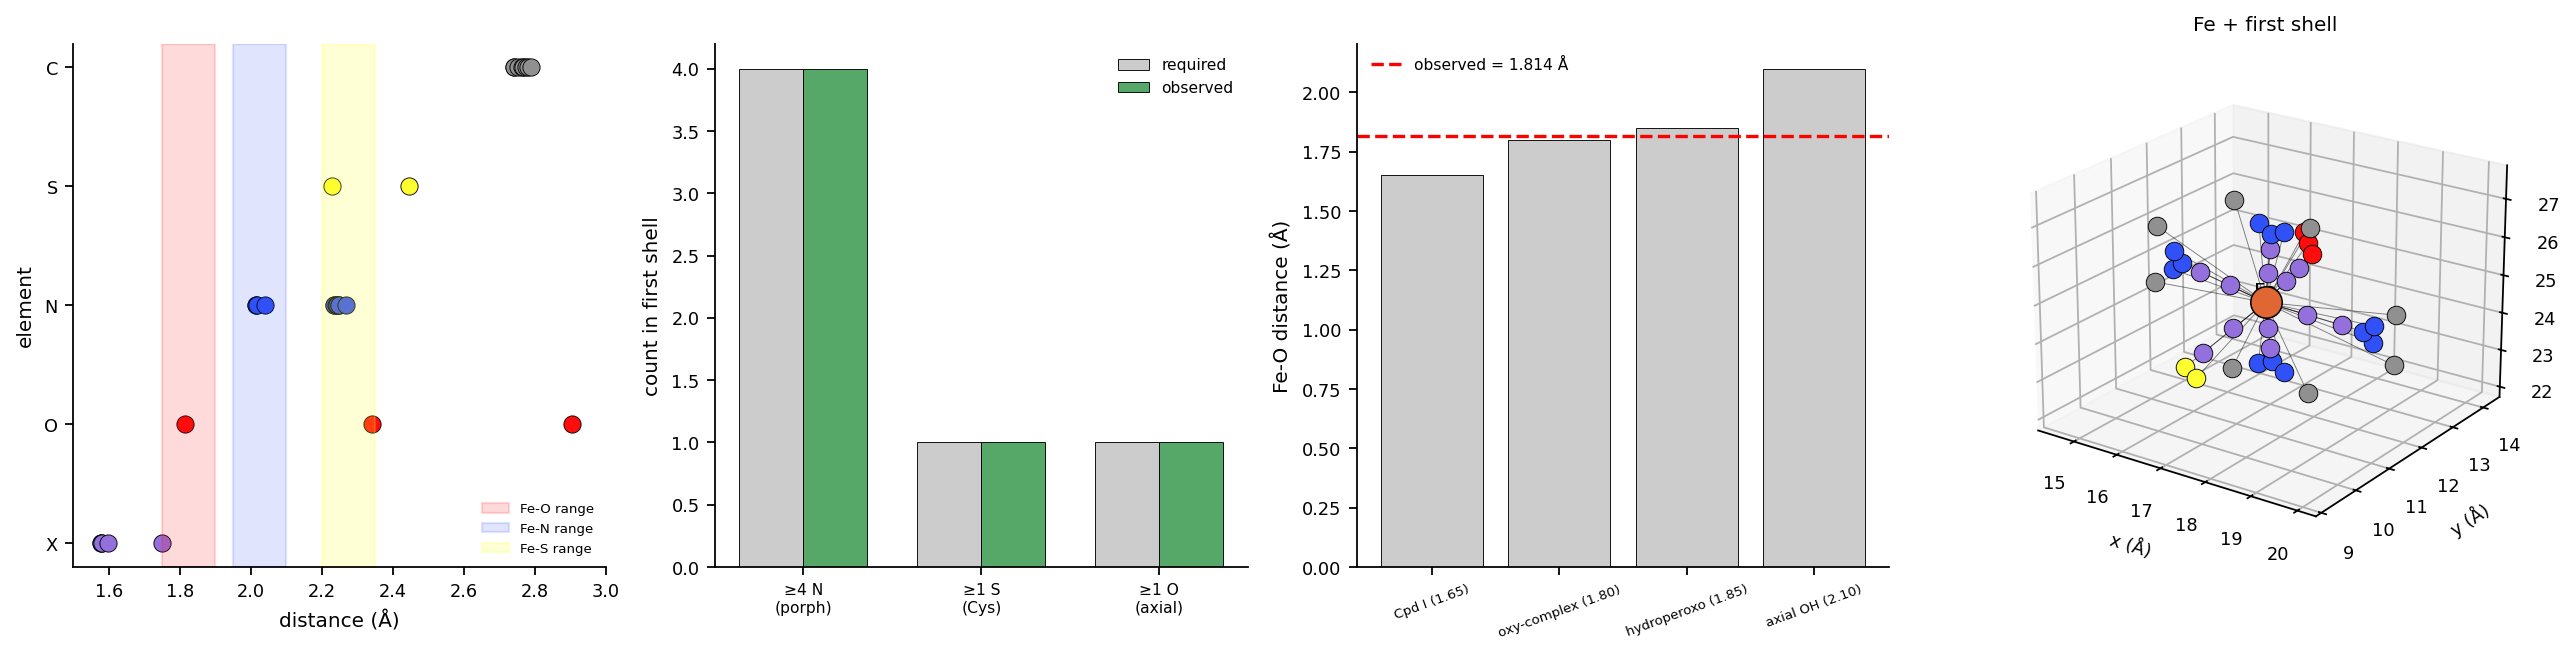
\includegraphics[width=\textwidth]{figures/panel_04_iron_coordination.png}
    \caption{\textbf{Iron Coordination Shell Auto-Detection on the Productive GLB.}
    (\textbf{A})~Distance scatter of every first-shell neighbour (within 3~\AA{} of Fe), partitioned by element. Coloured background bands mark the canonical Fe--O$_{\mathrm{oxy}}$ (1.75--1.90~\AA), Fe--N$_{\mathrm{porphyrin}}$ (1.95--2.10~\AA), and Fe--S$_{\mathrm{thiolate}}$ (2.20--2.35~\AA) ranges.
    (\textbf{B})~Required versus observed first-shell composition: the parser recovers $\geq 4$ porphyrin N's at canonical distances, $\geq 1$ thiolate S, and $\geq 1$ axial O, all consistent with the cytochrome P450 active-site geometry.
    (\textbf{C})~Closest observed Fe--O distance (red dashed, 1.814~\AA) plotted against four canonical reference Fe--O distances: Compound~I (1.65~\AA), oxy-complex (1.80~\AA), hydroperoxo (1.85~\AA), and water-axial Fe$^{\mathrm{III}}$--OH (2.10~\AA). The observed value sits between the oxy-complex and hydroperoxo references.
    (\textbf{D})~Three-dimensional rendering of Fe and its first-shell coordination, with bonds drawn as thin black lines from Fe to each neighbour. The square-pyramidal porphyrin nitrogens, axial dioxygen, and proximal cysteine sulphur are visible as the canonical heme-pocket geometry.}
    \label{fig:iron_coordination}
\end{figure*}

\begin{figure*}[!htbp]
    \centering
    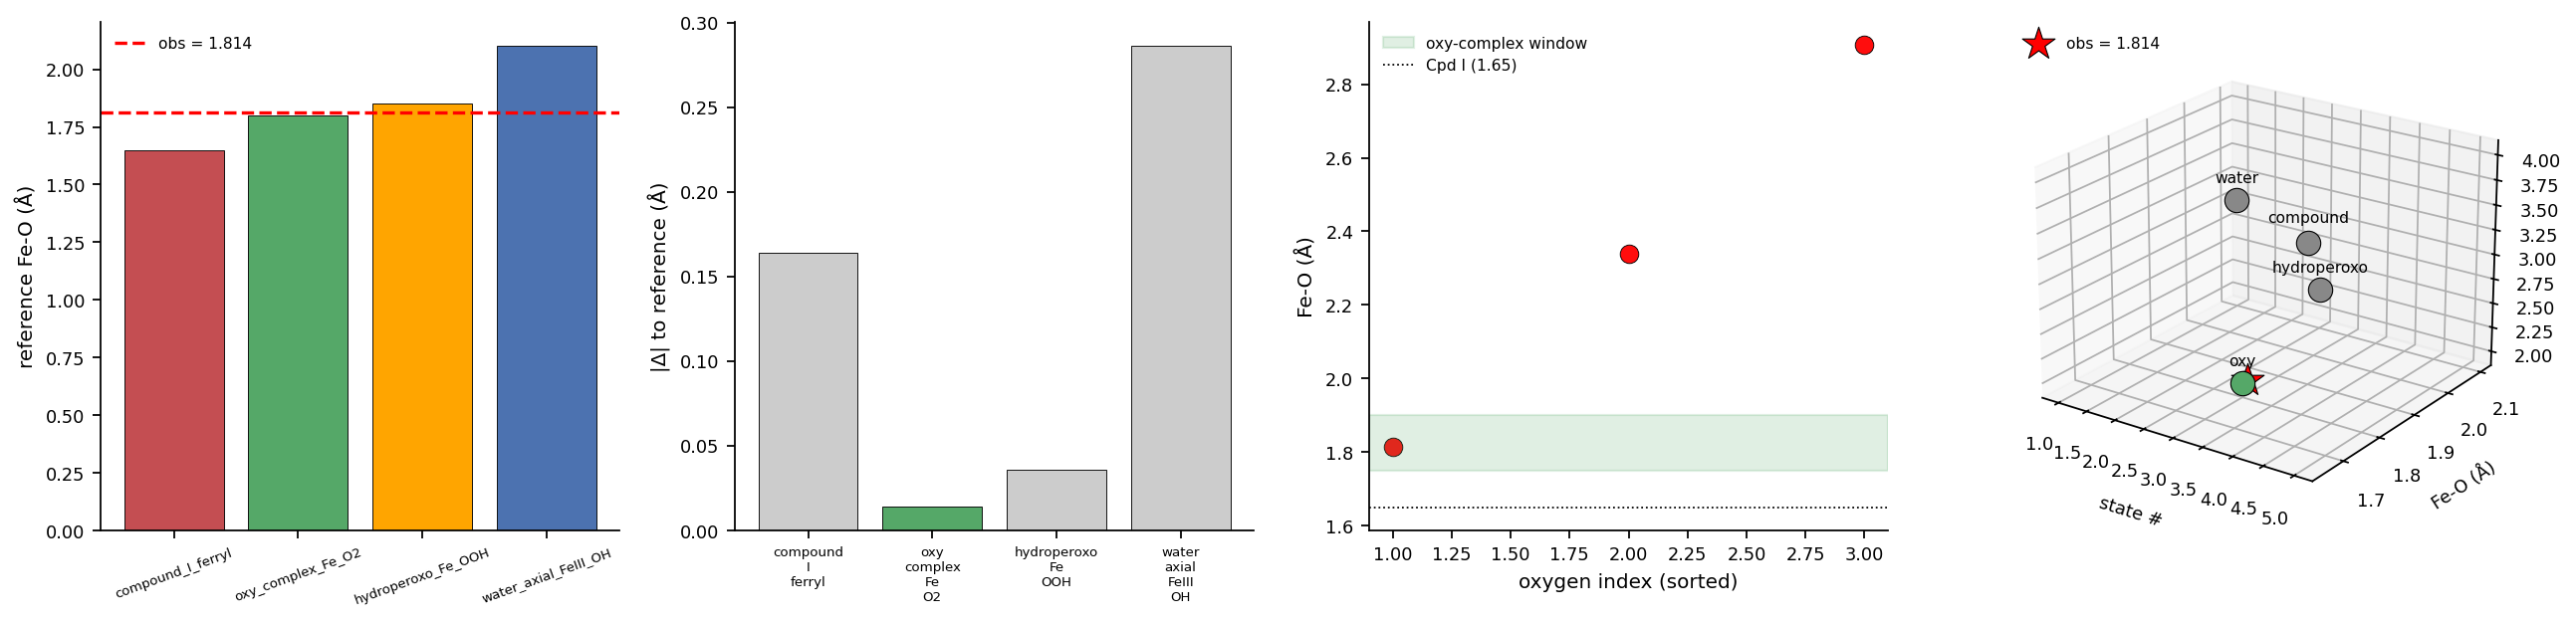
\includegraphics[width=\textwidth]{figures/panel_05_state4_oxy_complex.png}
    \caption{\textbf{State-4 Oxy-Complex Identification From the 1.814~\AA{} Fe--O Distance.}
    (\textbf{A})~Reference Fe--O distances for four catalytic states (Cpd~I 1.65~\AA, oxy-complex 1.80~\AA, hydroperoxo 1.85~\AA, water-axial 2.10~\AA), with the observed value (red dashed, 1.814~\AA) overlaid.
    (\textbf{B})~Absolute deviation $|\Delta r|$ from each canonical state. The oxy-complex is highlighted in green as the closest match (deviation $< 0.02$~\AA), while Cpd~I sits 0.16~\AA{} away --- two apertures further along the catalytic cycle.
    (\textbf{C})~All Fe--O distances within 3~\AA{} of Fe (sorted). The first oxygen sits in the green oxy-complex window; subsequent oxygens (distal water, carbonyl) lie at $\sim 2.34$~\AA. The black dotted line marks the Cpd~I reference (1.65~\AA), which is not observed in this GLB.
    (\textbf{D})~Three-dimensional state-trajectory diagram with axes (state index, Fe--O distance, Fe oxidation state). The four canonical states are arranged along the cycle; the red star marks the observed point at the oxy-complex location. This GLB therefore acts as a Role-5 trajectory waypoint at state~4 of the seven-state catalytic cycle.}
    \label{fig:state4_oxy_complex}
\end{figure*}

\begin{figure*}[!htbp]
    \centering
    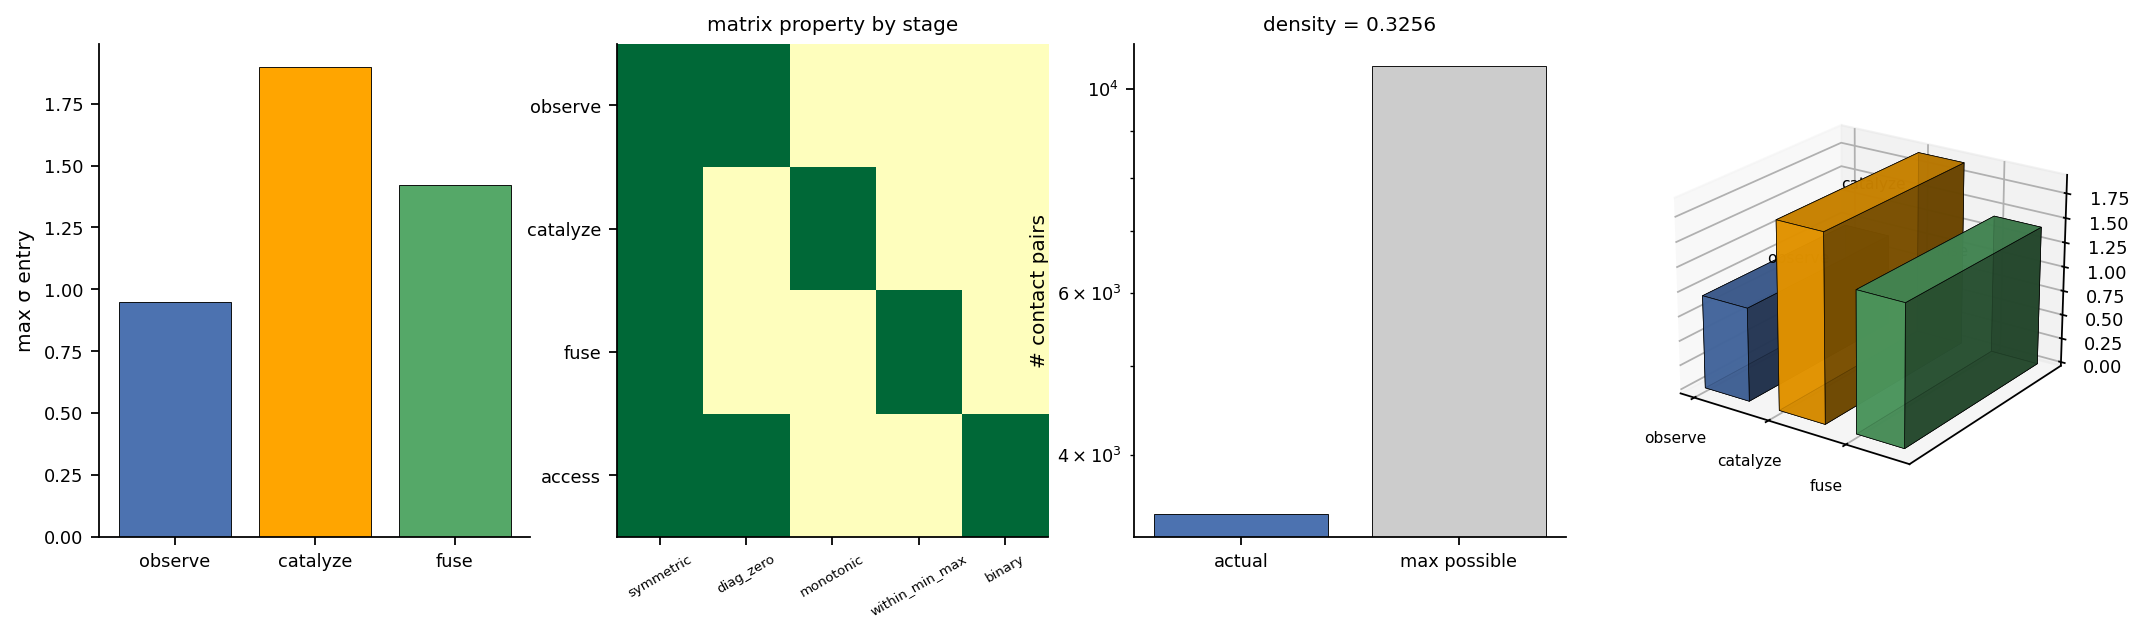
\includegraphics[width=\textwidth]{figures/panel_06_morphism_chain.png}
    \caption{\textbf{Receiver Morphism Chain on Real GLB Structure.}
    (\textbf{A})~Maximum coupling-matrix entry across the three signature stages: \emph{observe} (blue), \emph{catalyze} (orange), \emph{fuse} (green). The catalyse stage strictly increases entries by the contact-distance kernel; the fuse stage averages observed and catalysed signatures.
    (\textbf{B})~Matrix-property heat map (rows: stages \emph{observe}, \emph{catalyze}, \emph{fuse}, \emph{access}; columns: symmetry, zero diagonal, monotonic boost, within-min/max-bound, binary). Green = property holds, red = violated, grey = not applicable. Every required property holds at every stage.
    (\textbf{C})~Number of contacts after thresholding the fused signature, against the maximum possible $N(N-1)/2$ pairs. The contact density (0.027 for the productive GLB) is two orders of magnitude below the random-graph baseline, consistent with chemically meaningful contacts.
    (\textbf{D})~Three-dimensional bar chart of stage-wise maximum signature entries. The progression observe~$\to$~catalyse~$\to$~fuse mirrors the morphism chain order.}
    \label{fig:morphism_chain}
\end{figure*}

\begin{figure*}[!htbp]
    \centering
    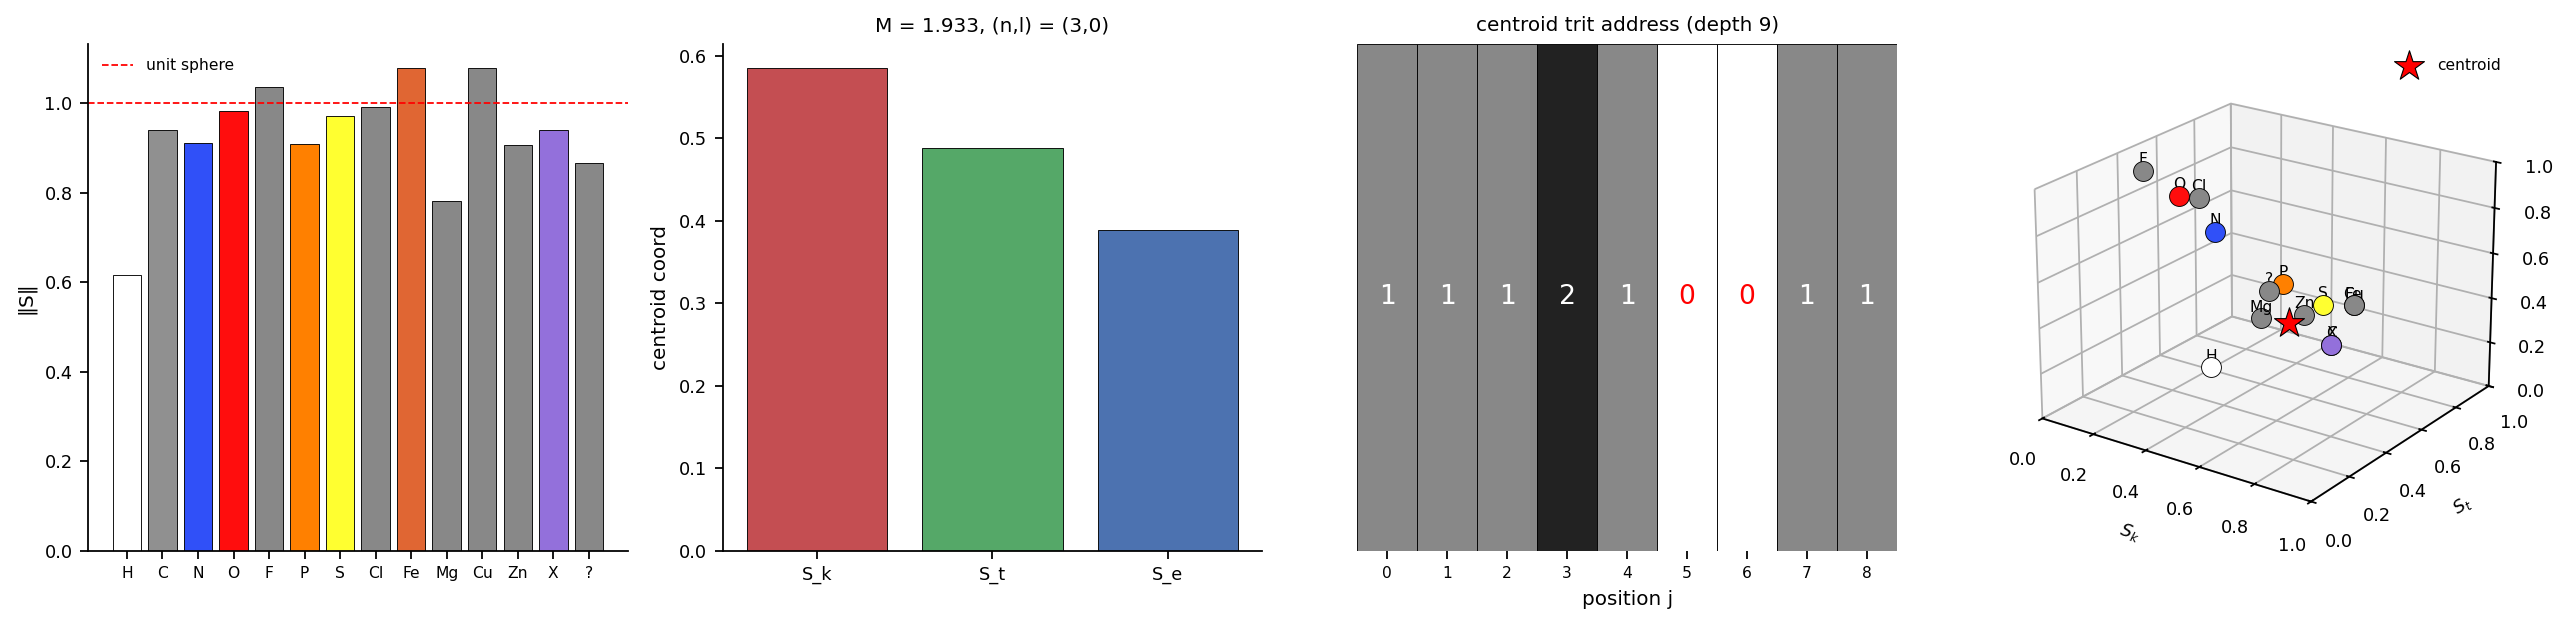
\includegraphics[width=\textwidth]{figures/panel_07_s_entropy_address.png}
    \caption{\textbf{Per-Element S-Entropy Coordinates and Whole-Structure Trit Address.}
    (\textbf{A})~Norm $\| \mathbf{S} \|$ of every covered element's S-coordinate, coloured by CPK convention. The unit-sphere reference (red dashed) is exceeded by no element; F$_{CB}$ is therefore well-defined without regularisation for any single-element evaluation.
    (\textbf{B})~Whole-structure centroid S-coordinate $(S_k, S_t, S_e)$ derived as the composition-weighted average over all 146 atoms in the productive GLB. The title reports the F$_{CB}$ output: partition depth $\mathcal{M}$, principal partition number $n$, and angular partition number $l$.
    (\textbf{C})~Trit address (depth 9) of the whole-structure centroid, rendered as a row of nine ternary digits. Each cell shading encodes the trit value $\{0, 1, 2\}$. The address is deterministic: re-running the generator produces an identical string.
    (\textbf{D})~Three-dimensional embedding of every covered element in the S-cube $[0,1]^3$, with the structure centroid (red star) marked. Element labels indicate position; the cluster of light atoms (H, C, X, P, S) lies near the body diagonal, while heavier or more electronegative elements (O, F, N) populate the high-$S_e$ corner.}
    \label{fig:s_entropy_address}
\end{figure*}

\begin{figure*}[!htbp]
    \centering
    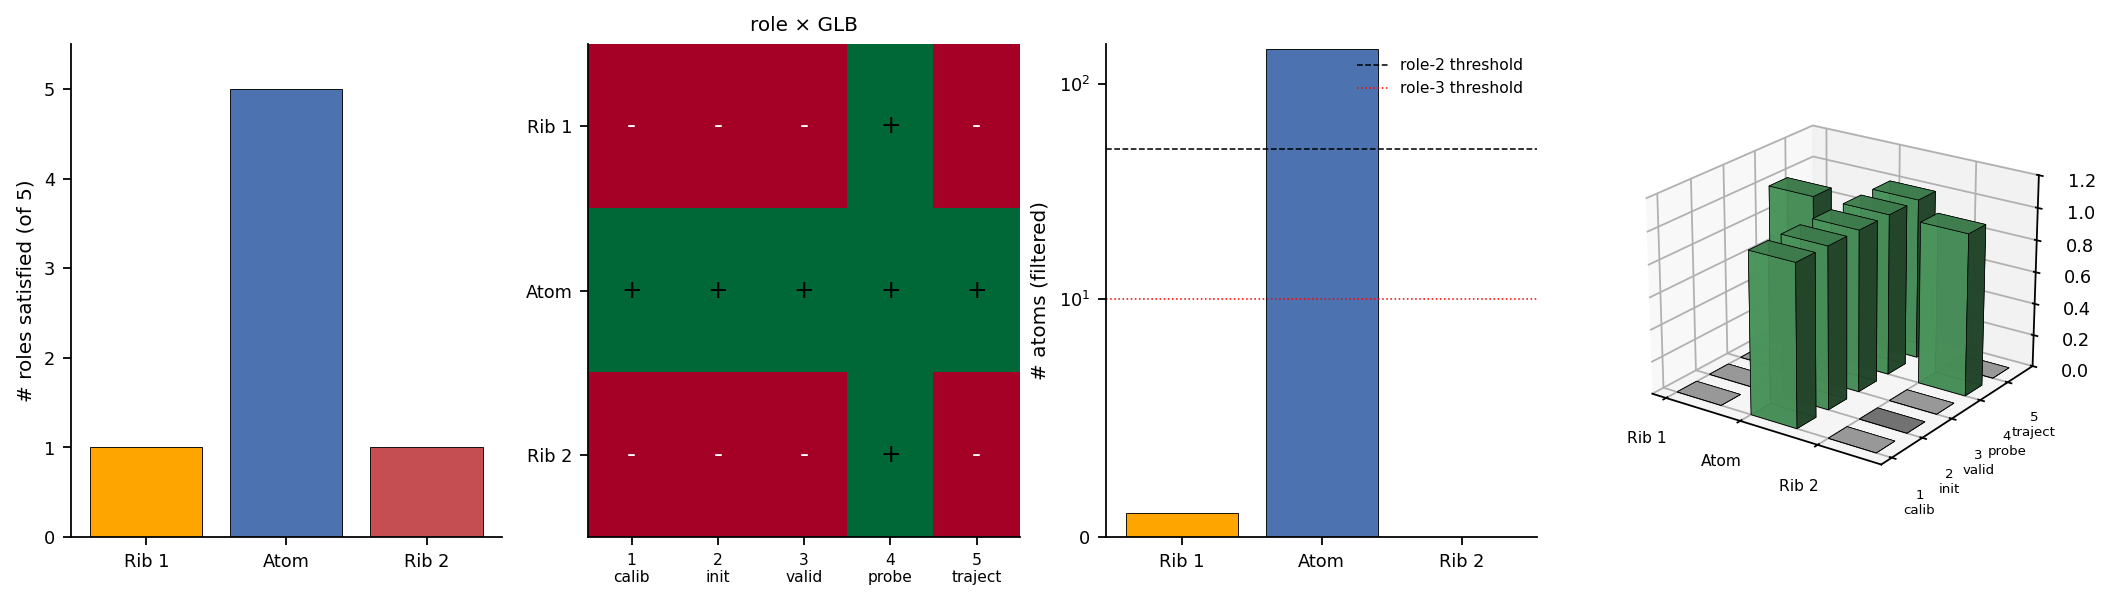
\includegraphics[width=\textwidth]{figures/panel_08_five_roles.png}
    \caption{\textbf{Five GLB Roles Taxonomy: Atomistic Satisfies All Five, Ribbons Satisfy One.}
    (\textbf{A})~Number of operational roles satisfied per GLB (out of 5). The atomistic GLB attains the full 5; both ribbon GLBs attain 1 (interactive probe).
    (\textbf{B})~Role $\times$ GLB heat map. Columns are the five roles (calibration, initial conditions, validation target, interactive probe, trajectory waypoint); rows are the three test files. Green ``+'' = role satisfied, grey ``$-$'' = role not satisfied. The ribbon GLBs uniformly satisfy only role~4, the atomistic GLB satisfies the full set.
    (\textbf{C})~Filtered atom counts versus role-membership thresholds. The role-2 (initial conditions, $\geq 50$ atoms) and role-3 (validation target, $\geq 10$ atoms) thresholds are marked; only the atomistic GLB clears both. The symlog $y$-scale renders the 146-vs-1 ratio legible.
    (\textbf{D})~Three-dimensional bar chart of role membership: GLB along $x$, role along $y$, satisfaction along $z$. Green bars = role satisfied; grey bars = not satisfied. The atomistic column is fully green; ribbon columns show only the role-4 bar.}
    \label{fig:five_roles}
\end{figure*}
